\documentclass{article}

\usepackage{amsfonts}
\usepackage{amsmath}
\usepackage{xcolor}

\title{research internship report}
\date{2018-28-01}
\author{Seppich,Nicolas}

\usepackage[backend=biber,sorting = none, style=numeric-comp, doi=false, isbn = false, url=false, giveninits=true]{biblatex}
\bibliography{Bibliography.bib}

\usepackage{pgfplots}
\pgfplotsset{compat=1.8,width = 5.5cm}
\usepgfplotslibrary{fillbetween}
\usepgfplotslibrary{groupplots}
\usepackage{pgfplotstable}
\usetikzlibrary{external}
%\tikzexternalize[prefix=./tikz/]


\begin{document}
{\bf Style guide}
\begin{itemize}
\item Treat equations as sentences, that is end them with point or comma's, so that it integrates with the text.
\item Focus on the content of the report, not the layout. That is for, don't try to force latex to have spacing at each paragraph. It is better to do this at the end, so you can programmatically perform these adjustments.
\item You have to ease the reader into the subject, assume that the person reading the text doesn't know anything about the report. Try to read it using this mindset and reflect if you would be able to follow your report when you had read it for the first time
\item Try to write it, so that you also enjoy it to read. If you don't enjoy it to read, don't expect that anyone else will like it either!
\end{itemize}
{\bf Suggestions for change}
\begin{itemize}
    \item Chapter 1 Preface and acknowledgment: Give here information on what you need the do for your university, why you choose the KTH and your part within the IMAGE project (keep the part about IMAGE short, there will be info later).
    \item Chapter 2 Introduction. Write here the background to the problem that you have looked at and explain the research objective.
        \begin{itemize}
            \item Background: Introduce the concept of acoustic liners, the measurement of their properties, connection with IMAGE and also introduce the prony method in words. Show that it works only for a equispaced grid. 
            \item Problem: Determine uncertainty in results obtained using Prony-like methods
            \item Objective: Introduce the use of non-equispaced grids
        \end{itemize}
    \item Chapter 3 Theory: Introduce here the information needed to understand the problem that you have worked on and focus on the approximation. Try to line up your writing with the code that you have used.
    \item Chapter 4 Results and conclusion
        \begin{itemize}
            \item Numerical experiments: Show here the results that you have obtained using your code and the error analysis that you have done.
            \item Experimental results: Show here the results that you have obtained using the uncertainty analysis.
        \end{itemize}
\end{itemize}


\maketitle
\pagenumbering{gobble}
\newpage
\pagenumbering{arabic}

\setcounter{secnumdepth}{5}

\section{Abstract}
As acoustics is field of studies that bother our everyday lives, it is important to distinguish between wanted and unwanted acoustics.
While on one side acoustics are highly appreciated and essential in the field of communication, noise on the other side is an unwanted side effects of many applications and can even lead to severe consequences for people.
Therefore, it is essential to develop efficient ways to reduce noise.

The research project, where I had the chance to get insights in during my internship covered the topic of passive noise reduction methodologies with acoustic liners in aircraft engines.
Since the fundamental principle of passive noise reduction with sound absorbing materials has been used for a long time, the focus is set on the optimization of several set ups.
That’s why I participated in experimental tests of new liner designs and as a main task worked on postprocessing of the obtained data, where my focus was set on recovering data at non equispaced positions and the approximation of underlying functions.
The main goal of the project is the creation of a data base associated with uncertainties as a reference for further optimization.  

\newpage 

\section{Introduction} 
Studying at university at undergraduate level usually means to a lot of students quite a theoretical education.
But since working in academia is supposed to combine both practical experimental and purely theoretical work, my department of the Technical University Munich provides the opportunity to gain insights into research topics during an optional research internship.
As part of my curriculum in engineering at the Munich School of Engineering, I decided to complete this internship at the Marcus Wallberg Laboratory for Sound and Vibration of the KTH in Stockholm, Sweden in the field of aero acoustics.
During the 6 weeks of the internship, I could support the researchers and gain a lot of insights in specific tasks, which I am going to present in the following pages.  

\subsection{The IMAGE project} 
The work I was included during the research internship was part of the so-called IMAGE- project, which stands for Innovative Methodologies and technologies for reducing Aircraft noise Generation and Emission.
This project aims to investigate noise reduction technologies in aircrafts both in a numerical and experimental way in order to develop robust methodologies in this particular field of study.  
The main goal of the study at the Marcus Wallenberg Laboratory is the characterization of the acoustical behaviour of porous materials in the reduction of fan noise.
As a fact, these porous materials are usually part of so called acoustic liners, which are used in aircraft engines, especially in turbofans to damp engine noise.
The obtained results provide the basis references for further optimization of liners or for further validation of numerical methods. 

\subsection{My field of activity} 
As the duration of the research internship was limited to period of 6 weeks, I participated in many tasks supporting the researchers instead of completing a single separate task.
These tasks are going to be explained in a detailed way in the following pages, but all in all encompassed the setup of experiments, research in literature, post processing the obtained data numerically with different methods and conducing an uncertainty analysis.
I worked both practically in the laboratory and theoretically on fundamental theories of acoustics and maths.
As a member of a team of 3, I could also benefit from the expertise of my colleagues as well as acquiring helpful skills in team working.
Fundamental theory and experimental setup
Basic theory concerning the experiment
Experimental setup and variation
\section{fundamental theory}
The field of acousitc covers quite a wide range of technical applications as already mentioned.
Basically, most phenomena can be deduced to a few simple relations, which are going to be presented subsequent. 
\section{Main topics processed during the internship}
\subsection{Gathering of information concerning acoustics } 
The first days of the internship were used to acquire the demanded knowledge about acoustics and its methodologies, that are descriped in the previous chaptor.
In order to fulfil this purpose, the main task was to read several books such as 1, 2, 3 and gather serveral articles concering this topic.
After a short period, I realized, that flow acoustics only is a combination of different subjects, which I already passed at TUM such as continuum mechanics, signal processing, control theory and thermodynamics.
With the acquired knowledge I was able to pass on to the main tasks. 
\subsection{Setup of the experiment and modifying parts}
Testing of new liners in the testing ricks, preparation of the liners, replacing, conduction of preliminary methods for the measurements, conduction of the first tests with/without flow

\subsection{Postprocessing data obtained by the experiments}

\subsubsection{Motivation/goals}
The main goal of the data post processing step is to determine the impedance of the acoustic liners, since the impedance can be seen as the main acoustical characteristic of a technical component.
This is done with the before mentioned complex relation between the wave number and the impedance.

{\color{red} You could introduce the relation between the wavenumber and impedance using an equation.
\begin{equation}
    k_y \tan 2k_y H = \frac{i \rho_0 c_0^2}{\omega z_{ac}} \left[k-M_zk_z\right]^2
\end{equation}
and
\begin{equation}
    k_z = \frac{k}{1-M^2} \left( -M \pm \sqrt{1+(1-M^2)(k_x^2/k^2 + k_y^2/k^2)}\right)    
\end{equation}
$k_z$ is measured, then from the first relation $k_y$ can be obtained under the consideration that the frequency is low enough that there are no modes in the $x$ direction $k_x = 0$, then with the first equation the acoustic impedance $z_ac$ can be obtained.

You can refer to this solution as the impedance obtained using the Ingmar-Myers boundary equation within a rectangular duct with uniform mean flow. See also the theory pdf}


As measured data is always accompanied by uncertainties, it is also of high importance to fit the uncertainty analysis into the basic modelling process.
Normally, this is a problem of non-trivial kind based on the right assumptions.
With the initial situation of only a few measurement points with quasi equispaced distances it is not possible to calculate uncertainties, where derivatives in the following form are demanded:
\begin{equation}
u_{i}(q)= \left\vert \frac{\partial q}{\partial x_{i}} \right\vert u( x_{i})
\end{equation}
where $u_{i}(q)$ denotes the uncertainty in the desired quantity $q$ due to the uncertainty in $x_{i}$.

{\color{red} Move this after the Prony Using the fact, that the microphone postitions are not perfectly equispaced, allows us to approximate the wanted function at equipaced steps.
Thus, new data points are generated, which are not only necessary to calculate derivatives, but also to use the Prony method, where an equispaced grid is a basic requirement. }

\subsubsection{Introduction to the Prony method}
In this section, the already mentioned Prony method is shortly introduced, which aims to recover the signal parameters from noisy sampled data to determine the experimental impedance of the liners.
{\color{red} Write that the acoustic field within the line duct consists of acoustic modes and the general form is given by \ref{eqn: expsum}. Say that when the factors $c_j$ and $k_j$ are known, they can be related to the acoustic impedance with the previous equations} 
So, the problem that we were faced to solve can be considered as a nonlinear approximation problem of the form:
\begin{equation}\label{eqn: expsum}
 p(x)=\sum\limits_{j=1}^M c_{j}e^{ik_{j}x} 
\end{equation}
where the pairwise different wavenumbers $k_{j}$ and complex coefficients $c_{j}$ are recovered.

{\color{red} The following paragraph is too vague and hard to follow. Just write that there is a algebraic solution to the above problem, also known as the prony method. Say that there are various prony-like methods and refer to Potts. Say that in order to have an algebraic solution, it is necessary that data is obtained at M*2 data points and that these are equispaced. Refer back to the problem statement of the uncertainty analysis and argue that the microphone positions will never be equispaced. Thereafter introduc the algorithm outlined in the article as a solution to the problem}

The problem is solved using methods like the singular value decomposition of a generated Hankelmatrix consisting of the complex pressures $p(x)$ and the solution of an overdetermined Vandermode System.
The detailed implementation of the prony method was the main task of my colleague.
Therefore, advanced tecnical information about the method are not going to be provided in this context.
But nevertheless, it's essentiell to know the basic ideas of the method for a better understanding the subsequentiell steps. 


\subsubsection{Equispacing algorithm}
{\color{red} Here you don't have to write what your task was, this should be written in the very beginning. You should here make it clear that you implemented the algorithm by Peter and explain the functioning of the algorithm. Try to write this as clear as you can, you should be the expert by now! (Otherwise the reader will wonder what you have done or really understand if you can't explain it clear}
For the purpose to use the prony method precisely as well as using uncertainty estimates, it was necessary to implement an eqispacing algorithm. 
To develop this algorithm, which approximates the unknown function of complex pressures at equispaced positions and to understand the mathematical theory behind it, was basically my main task to be completed during the internship.
It occupied also most of the time.
The algorithm is based on the \textit{non linear approximation by sums of exponentials and translates}, by “Peter, Pots and Tasche”. \cite{Peter2011} 

To enhance the understanding of the sequential formulas, the main parameters of the algorithmn are going to be presented in the following:
\\\\
 K: K is the number of nodes and therefore the number of rows in the following linear equation\\
 N: N is the nonharmonic Bandwidth\\
 L: L is the number of exponentials to approximate the function
\\\\
The basic idea of the algorithm is as before in equation \eqref{eqn: expsum} to approximate the function of obtained complex pressures with a linear combination of comlex exponentials.
In this case, we generalize the equation \eqref{eqn: expsum} to a nonequispaced grid, i.e. on the known nodes $x_{k}\in (k=1,...,K)$ with the sampled data  $p(x_{k}) $
\\
\begin{equation}
 p(x)=\sum\limits_{j=1}^L c_{j}e^{2\pi ixNs_{j}}
\end{equation}
where N denotes the non harmonic bandwidths and with complex coefficients $c_{j}\neq0, x_{k} \in (-\frac{1}{2},\frac{1}{2})$.

But in order to recover the parameters of the sum,the signal must be brought into the form first:  
\begin{equation}\label{eqn:truncatedw}
 p(x)=\sum\limits_{j=1}^L h_{l}\psi(x-\frac{l}{L})
\end{equation}

Where $\psi$ denotes the so called truncated window function with many helpful properties such as to be localised well in space and time, which will be discussed later more detailed. \\

\paragraph{Window functions	} $ $\\[1ex]
In general, a function is called a window function, which is zero valued outside a specific chosen interval.
So as one can assume, there are quite a lot of possibilities to set up these window functions.
For our case the 1- periodization of a gaussian bell, as proclaimed in the paper of Steidl seemed to provide good results to work on with.
It is of the form: 

For a fixed $b>0$ and L let:
\begin{equation}
\varphi(x)= \frac{1}{\sqrt{\pi b}} \sum\nolimits_{r \in \mathbb{N}}  e^{(L(x+r))^2/b}
\end{equation}
The truncated version of the gaussian bell takes the form: 
\begin{equation}
\psi(x)= \frac{1}{\sqrt{\pi b}} \sum\nolimits_{r \in \mathbb{N}}  e^{(L(x+r))^2/b}\chi_{(-m,m)}(L(x+r))
\end{equation}
with $1<m < \frac{L}{2}$ and
\begin{equation}
    \chi_{(-m,m)}(x)=
    \begin{cases}
      0, & \text{if}\ x\in (-m,m) \\
      1, & \text{otherwise}
    \end{cases}\notag
\end{equation} 
The question arose, why do we need to truncat the Gaussian bell? In the end, this is a mathematical trick to be well localized in space and time, which allows further mathematical proofs, that are not examined in this report further on.

So, after setting up the truncated window function we are able to solve the linear systems of equations of this form:
\begin{equation}
\sum\limits_{j=1}^L h_{l}\psi(x_{k}-\frac{l}{L})=p(x_{k})
\end{equation}
This can be written in a linear system of equations, which can be solved easily. {\color{red} You could write the matrix equation, just to make it easier to follow}
Here, we aim to examine the coefficients $h_{l}$, which will be used in the second step to approximate the function on the equispaced grid at the specific positions.
The grid can be equalized, using a simple algorithm, which examines the average step size and generates a new grid with this information.
With all coefficients $h_{l}$ and equipspaced positions $x'_{l}$ it is now possible to examine to approxiamte the complex pressure at the equispaced grid. 
\begin{equation}
 \sum\limits_{j=1}^L h_{l}\psi(x'_{k}-\frac{l}{L})=p(x'_{k})\notag
\end{equation}

\paragraph{Results using the truncated window function} $ $ \\[1ex]
In the following, the results of this specific method are going to be discussed.
The parameters where chosen by formulas presented by Peter: \\
	(formulas for parameters) \\
	(graphs)
As the results show, the approximation of the function worked well within the domain, but diverged on the boundaries.
So, using the truncated window function in this specific case was not the optimal solution. \\[1ex]

\paragraph{Approximation with a single Gaussian Bell}  $ $ \\[1ex]
The major goal of the algorithm is to approximate the function of complex pressures as good as possible.
Due to the fact, that every function can be approximated by almost any function, we slightly changed our startin function \eqref{eqn:truncatedw} {\color{red} Why? Explain!} and simply used this form of the original gaussian window function: 
\begin{equation}
 p(x)=\sum\limits_{j=1}^L h_{l}\varphi(x-\frac{l}{L})
\end{equation}
with $\varphi$ is the orignal gaussian bell function: 
\begin{equation}
\varphi(x)= \frac{1}{\sqrt{\pi b}}  e^{x^2/b}
\end{equation}
where l denotes the shift parameter.

In essence, the rest of the main algorithm remained basically the same.
It is still the goal to deduce the coefficients $h_{l}$ by solving the linear system of equations: 
\begin{equation}
\sum\limits_{j=1}^L h_{l}\varphi(x_{k}-\frac{l}{L})=p(x_{k})
\end{equation}
and then approximate the function with remained coefficients at the equispaced grid: 
\begin{equation}
 \sum\limits_{j=1}^L h_{l}\varphi(x'_{k}-\frac{l}{L})=p(x'_{k})\notag
\end{equation}
Again, the algorithm needed to be verified under realistic values and under a nonequispaced grid. A testclass with possible numbers of scenerios. 
During the test cases with using error estimation techniques, it could be examined that the algorithm fulfilled the proclaimed purpose as long as the nonequispacing was not set to random {\color{red} If you have information on the limitations of the mind, include it! This will strengthen your belief that it works for the cases for which we are using the algorithm for}

\begin{figure}[b]% Reflection coefficient   
    \centering
    \begin{tikzpicture}[scale = 1]
        \begin{axis}[
                xlabel={Frequency [kHz]},
                ylabel={$|\hat{\mathcal{R}}|$ [-]},
                axis on top,
                xmin = 0, xmax = 4,
                ymin = 0.96, ymax = 1,
                minor tick num = 5,
                grid
            ]
            \addplot[
                    color =  red,
                    line width = 0.5,
                ] 
                table[x expr= \thisrow{f}/1000, y={mag} ] {./Data/UncertaintyAnalysis.txt};
            \addplot[line width = 1] table[x expr= \thisrow{f}/1000, y={create col/linear regression={y=mag}}] {./Data/UncertaintyAnalysis.txt};
        \end{axis}
    \end{tikzpicture}
    \begin{tikzpicture}[scale = 1]
        \begin{axis}[
                xlabel={Frequency [kHz]},
                ylabel={$\angle \hat{\mathcal{R}}$ [deg]},
                axis on top,
                xmin = 0, xmax = 4,
                ymin = -5, ymax = 5,
                minor tick num = 5,
                grid
            ]
            \addplot[
                    color =  black!90,
                    line width = 0.5,
                ] 
                table[x expr= \thisrow{f}/1000, y={phase} ] {./Data/UncertaintyAnalysis.txt};
        \end{axis}
    \end{tikzpicture}
    \caption{Measured reflection coefficient of the rigid plate. In blue the measured value and red gives the 95\% confidence intervals}
    \label{fig:ReflCoeff}
\end{figure} 

\begin{figure}
\centering
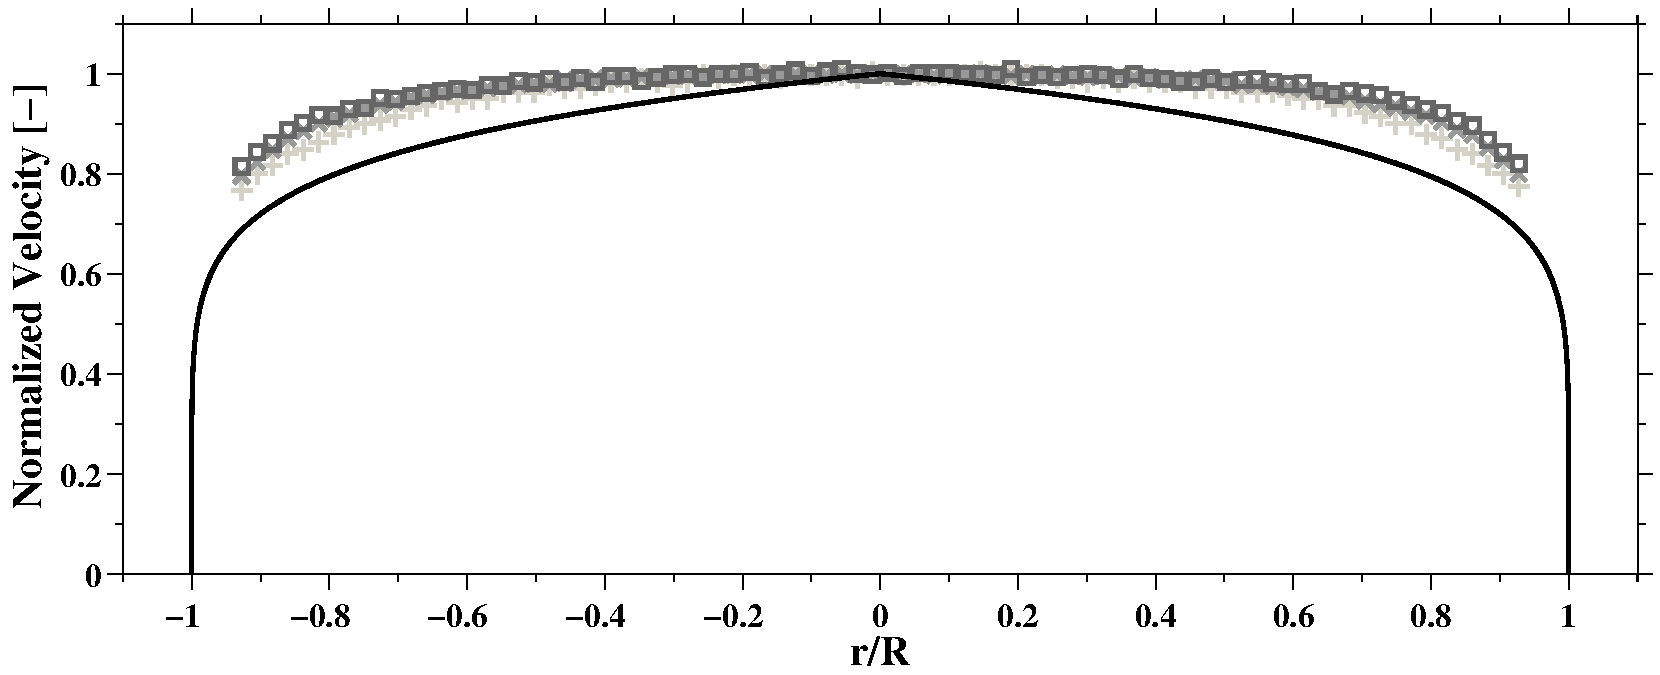
\includegraphics[width = 0.8\textwidth]{./Figures/FlowProfile_Large}
\caption{Test 123}
\end{figure}

\cite{Peter2011}
\cite{Mungur1969}
\printbibliography

\end{document}
